\chapter{Metodologia do trabalho}
\label{CAP3}

Esta seção trata das fases do trabalho: como foram  executadas e em que sequência.

% descrever fases do trab: concepcao, projeto, implementacao, testes
% (falar com o prof)


\section{Coleta de dados via celular}
Para coletar dados de aceleração, é possível utilizar os sensores embutidos nos \textit{smartphones}. Através de aplicativos móveis desenvolvidos para este fim, é viável interagir com os acelerômetros do dispositivo. Esses sensores registram a aceleração em relação aos eixos x, y e z. 


\begin{figure}[hp]
    \centering
    
    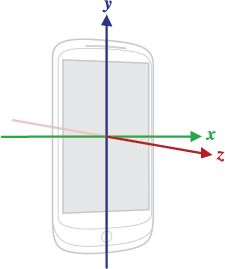
\includegraphics[]{figures/axis_android_device.png}
    
    \caption{Sistema de coordenadas que rege os valores dos acelerômetros de um dispositivo Android\textsuperscript{[27]}.}
    
    \label{fig:axis_android}
\end{figure}

Ao integrar esse aplicativo ao sistema, é possível obter informações detalhadas sobre a aceleração do veículo em que o \textit{smartphone} está instalado. A taxa de amostragem desses dados pode ser ajustada para atender às necessidades específicas do sistema por um parâmetro chamado \textit{minMillisBetweenData} no repositório do \textit{GitHub} https://github.com/APF2000/android-obd-reader-pires. 

Posteriormente, os dados coletados foram armazenados e processados para análises mais aprofundadas, contribuindo para a avaliação do comportamento de condução e identificação de padrões. Essa abordagem, aproveitando os recursos dos \textit{smartphones}, oferece uma solução prática e acessível para a coleta de dados de aceleração.

A figura \ref{fig:aceleracao} mostra os gráficos da aceleração a partir dos dados coletados do celular. 

A relação entre o gráfico da aceleração e uma curva feita pelo carro é fundamental para compreender o comportamento dinâmico do veículo durante a condução. No contexto da física do movimento, a aceleração é a taxa de variação da velocidade em relação ao tempo. Quando um carro realiza uma curva, ele experimenta uma aceleração centrípeta, que é direcionada para o centro da curva. Isso significa que a aceleração varia em magnitude e direção conforme o veículo percorre a curva.

Em um gráfico típico de aceleração durante uma curva, a forma da curva no gráfico pode fornecer informações sobre a suavidade da curva, a intensidade da aceleração lateral e até mesmo indicar a presença de manobras abruptas. Curvas suaves geralmente se refletem em padrões de aceleração mais graduais, enquanto curvas mais acentuadas ou manobras rápidas podem resultar em picos agudos no gráfico.

Essa relação entre o gráfico de aceleração e a curva feita pelo carro é valiosa não apenas para entender a dinâmica do veículo, mas também para avaliar a qualidade da condução. O Sistema de coleta de informaões de veículos que incorporam a análise desses dados podem oferecer insights importantes sobre o estilo de direção, ajudando na identificação de comportamentos agressivos, curvas perigosas ou necessidade de aprimoramento nas habilidades de condução. 

Essa integração contribui para a segurança e eficiência do sistema de rastreamento, proporcionando uma compreensão mais completa do desempenho do veículo em diferentes cenários de condução. A figura \ref{fig:sudden_acc_car} ilustra como essa análise pode ser feita.

\begin{figure}[hp]
    \centering
    
    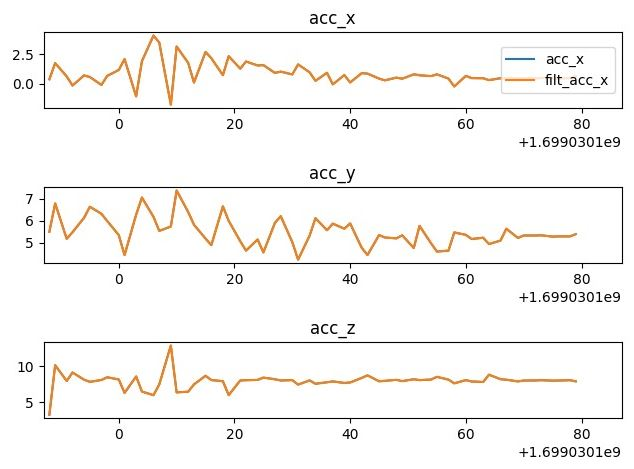
\includegraphics[scale=0.8]{figures/acelaracao.jpg}
    
    \caption{Gráfico da aceleração nos eixos x, y, z.}
    
    \label{fig:aceleracao}
\end{figure}

\begin{figure}[hp]
    \centering
    
    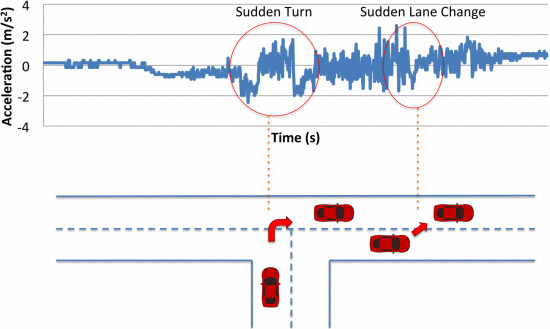
\includegraphics[scale=0.6]{figures/sudden_acc_car.jpg}
    
    \caption{Correspondência entre variações de aceleração e movimentos relativos do carro\textsuperscript{[15]}.}
    
    \label{fig:sudden_acc_car}
\end{figure}

\section{Transferência de dados para a nuvem e estruturação}

A transferência de dados para a nuvem e a sua estruturação desempenham um papel crucial na eficiência e escalabilidade do sistema de rastreamento de veículos. Ao adotar uma abordagem baseada na nuvem, os dados coletados, como informações de localização e padrões de condução, podem ser transmitidos de maneira eficiente para servidores remotos, proporcionando uma centralização dos dados. A estruturação desses dados na nuvem envolve a organização lógica e eficaz das informações em bancos de dados, facilitando a recuperação e análise posterior. 

A utilização de serviços de armazenamento em nuvem, no caso de projeto foi utilizado o AWS RDS, permite não apenas a transferência segura dos dados, mas também a flexibilidade de expansão conforme a quantidade de informações aumenta. Assim, a estruturação adequada dos dados na nuvem é fundamental para suportar consultas eficientes, análises e integrações com outras ferramentas, contribuindo para a tomada de decisões informadas e aprimoramento contínuo do sistema de rastreamento de veículos. 

Essa abordagem na nuvem oferece uma solução escalável e resiliente, garantindo que o sistema possa crescer de maneira sustentável e proporcionar \textit{insights} valiosos ao longo do tempo.

\section{Geração dos dados}
Ao incentivar voluntários a conduzirem por diferentes áreas do bairro, é possível coletar dados valiosos sobre o modo de direção de vários motoristas.

A diversidade de percursos percorridos por motoristas voluntários contribui para a construção de um mapa de rota abrangente e atualizado. Essa abordagem colaborativa enriquece a base de dados do sistema, mas também cria um senso de comunidade ao envolver os residentes no aprimoramento das informações de navegação locais. A figura \ref{fig:rota} ilustra como essa análise pode ser feita.

\begin{figure}[hp]
    \centering
    
    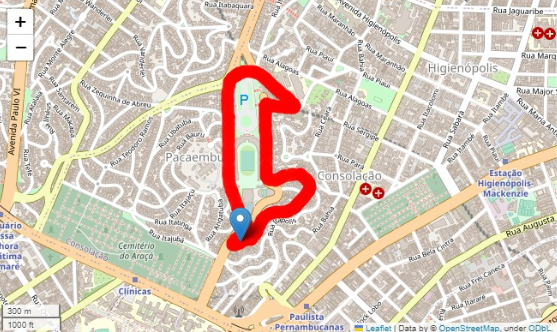
\includegraphics[scale=0.6]{figures/rota.png}
    
    \caption{Rota feita por um dos integrantes do grupo ao redor do seu bairro.}
    
    \label{fig:rota}
\end{figure}

\section{Visualização dos dados}
A análise de dados no contexto deste projeto pode ser eficientemente conduzida utilizando o \textit{Jupyter Notebook}, uma poderosa ferramenta interativa para análise de dados e programação em \textit{Python}. Ao importar os conjuntos de informações coletadas pelo sistema para o Jupyter Notebook, é possível explorar, visualizar e interpretar os dados de maneira flexível. 

A variedade de bibliotecas de análise de dados em Python, como Pandas, NumPy e Matplotlib, podem ser aplicadas para realizar operações estatísticas, identificar padrões de comportamento do motorista e gerar visualizações informativas. A combinação da facilidade de codificação do Python com a interface interativa do Jupyter Notebook permite a criação de análises exploratórias e gráficos informativos  para identificar tendências ou comportamentos específicos dos motoristas.

Dessa forma, o Jupyter Notebook emerge como uma ferramenta essencial para a compreensão aprofundada dos dados coletados, contribuindo significativamente para insights valiosos no contexto do sistema de rastreamento de veículos.

\section{Análise dos dados}
A análise de dados se torna uma jornada dinâmica e poderosa quando é combinado o AWS RDS (Relational Database Service) e o Jupyter Notebook. Ao armazenar os dados do sistema de rastreamento de veículos no AWS RDS, foi uma infraestrutura segura e escalável para a gestão eficiente de grandes volumes de informações dos parâmetros utilizados para analise. 

A integração com o Jupyter Notebook permite a exploração dos dados de maneira interativa e colaborativa. Ao estabelecer uma conexão direta entre o Jupyter Notebook e o banco de dados RDS, pode-se executar consultas SQL diretamente no ambiente de notebook, extrair conjuntos de dados relevantes e realizar análises exploratórias utilizando bibliotecas poderosas como Pandas e Matplotlib. 

A combinação dessas ferramentas facilita a visualização de tendências, identificação de padrões e até mesmo a implementação de algoritmos de aprendizado de máquina para prever comportamentos de condução. Essa sinergia entre AWS RDS e Jupyter Notebook não apenas agiliza o processo de análise de dados, mas também contribui para insights acionáveis que impulsionam a tomada de decisões informadas no aprimoramento contínuo do sistema de rastreamento de veículos.

Conforme o artigo citado anteriormente (\textit{Driver behaviour profiling using smartphone sensory data in a V2I environment}\textsuperscript{[15]}), é possível usar métricas de movimentação brusca do carro para classificar motoristas segundo a segurança de sua direção.

Mais especificamente, o estudo determina quatro tipos de condutores: muito cautelosos, cautelosos, agressivos e muito agressivo\textsuperscript{[15]}.

A classificação depende basicamente de quantos movimentos bruscos são feitos e em que situações eles ocorrem. Isso significa que em um ponto de maior convergência de estradas, por exemplo, haverá maior penalidade para o \textit{driver safety index} que em um local de menos movimento ou.

Dessa forma, esse estudo procura ranquear melhor os motoristas que têm menos probabilidade de gerar acidentes.

\section{Simulador de OBD}
O uso do simulador de OBD (On-Board Diagnostics) representa uma ferramenta valiosa no desenvolvimento e teste de sistemas de rastreamento de veículos. Este simulador emula as funcionalidades de um veículo, permitindo que os desenvolvedores testem a integração de seus sistemas de rastreamento sem a necessidade de um carro real.

Ao emular dados típicos como velocidade, rotações por minuto (RPM), temperatura do motor, e outros parâmetros do OBD, o simulador cria um ambiente controlado para verificar a eficácia do sistema em diferentes cenários de condução. Isso possibilita testes abrangentes, desde a coleta de dados até a análise de comportamentos específicos, garantindo a robustez e confiabilidade do sistema de rastreamento.

Além disso, o uso do simulador de OBD permite a realização de testes de maneira repetitiva e consistente, fornecendo dados padronizados para avaliação de desempenho e detecção de possíveis problemas antes da implementação em um ambiente de produção. 